\item Performance requirements:

Requirements for the Buzz system were for non-reporting operations to preferably not last longer than 0.2 seconds and for report queries to be processed in no more than 5 seconds.
To test this we used Firebug, an open source web browser extension of Firefox used for webpage monitoring. (Version used: Firebug 2.0.7).
The Buzz system met these requirements:
\begin{itemize}
\item Non-reporting operations such as returning to a previous page (i.e. operations that relied on cached copies of a web page) completed relatively close to the target time limit (e.g. returning to the main Buzz Spaces page after viewing the user’s profile took only 0.286 seconds, very close to the target time of 0.2 seconds).

\begin{figure}[h!]
  \centering
    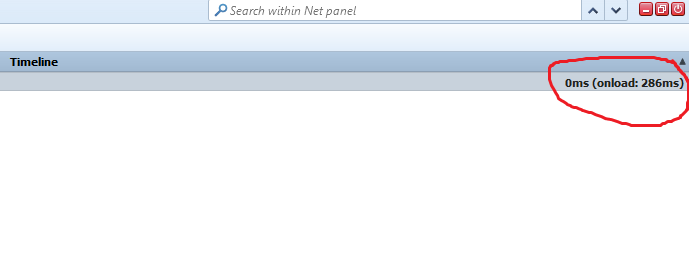
\includegraphics[width=0.85\textwidth]{Non-reporting_operationB}
    \caption{Non-reporting operation test}
\end{figure}

\item Report query operations (i.e. which had to communicate and receive some information from the system’s database) also completed within their desired time limit of 5 seconds (e.g. accessing the test module “TEST443”’s discussion space took only 1.24 seconds). Even some of the report query operations which took comparatively long to complete stayed within the 5 second limit (e.g. accessing module “COS332” took 4,81 seconds and accessing the Admin tab took 4,96 seconds).

\begin{figure}[h!]
  \centering
    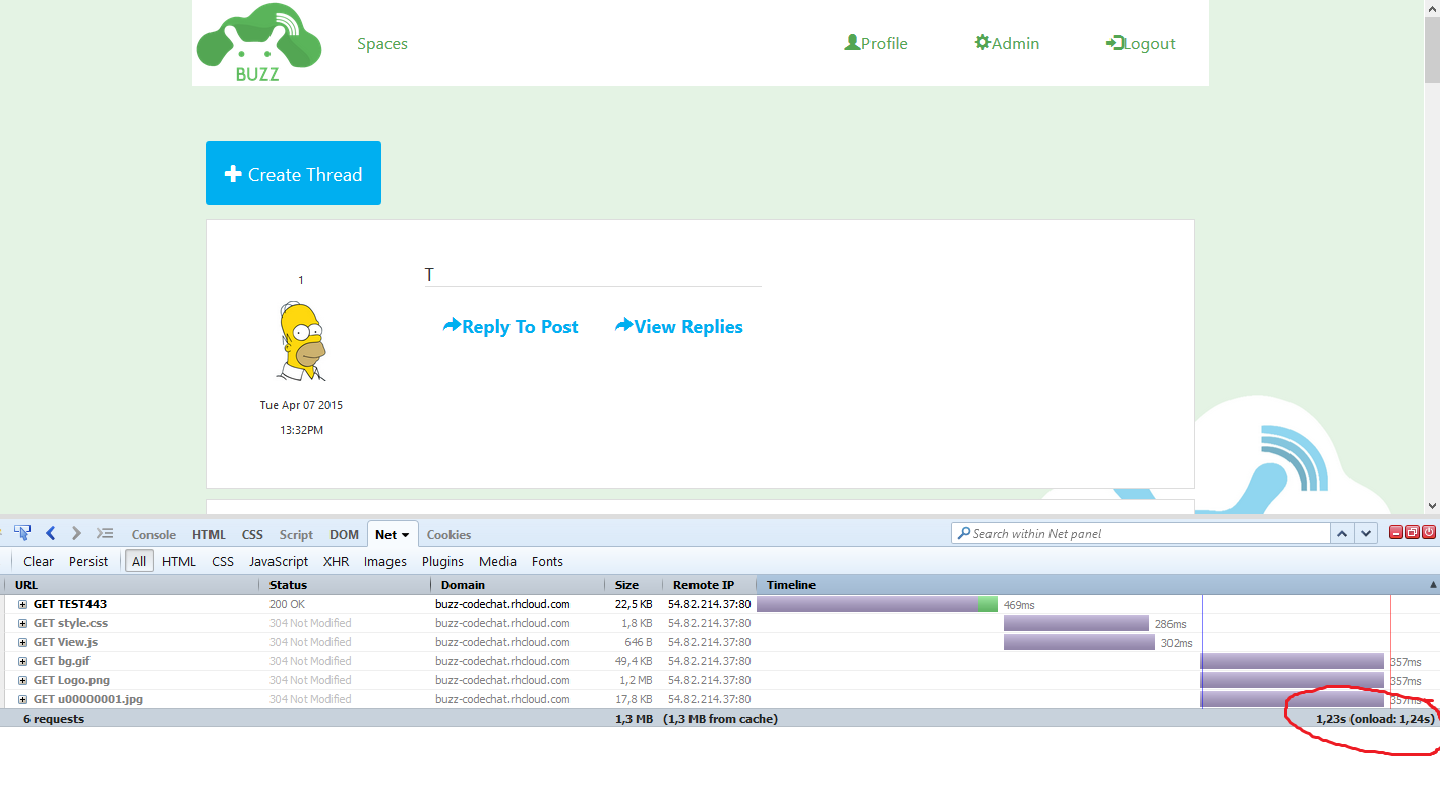
\includegraphics[width=0.85\textwidth]{Reporting_operationB}
    \caption{Reporting operation test}
\end{figure}

\end{itemize}	
